\documentclass[a4paper,12pt]{article}
\usepackage[utf8]{inputenc}
\usepackage{enumitem}
\usepackage[T1]{fontenc}
\usepackage{amssymb}
\usepackage{graphicx}
\usepackage{pstricks}
 \usepackage{amsthm}
 
%\usepackage[nohead]{geometry}
%\usepackage{amsmath,amsthm,amssymb,euler}

% \newtheorem{deff}{Definicja}[subsection]
% \newtheorem{twr}[deff]{Twierdzenie}
% \newtheorem{lem}{Lemat}
% \newtheorem{uwaga}[deff]{Uwaga}
% \newtheorem{alg}[deff]{Algorytm}
 \usepackage{algorithm}
\usepackage{algorithmic}
%Change: REQUIRE -> Input and ENSURE -> Output
%\renewcommand{\algorithmicrequire}{\textbf{Input:}}
%\renewcommand{\algorithmicensure}{\textbf{Output:}}


\newtheorem{deff}{Definition}[subsection]
\newtheorem{theorem}{Theorem}
\newtheorem{lem}{Lemma}
\newtheorem{uwaga}[deff]{Remark}
\newtheorem{alg}[deff]{Algorithm}

%\newcommand{\e}[0]{\mathbf{e}}
%\newcommand{\s}[0]{\mathbf{s}}
%\newcommand{\PP}[0]{\mathbf{P}}
%\newcommand{\E}[0]{\mathbb{E}}
 
\renewcommand\theequation{\thesection.\arabic{equation}}
%\setlength{\textwidth}{16cm}
%\setlength{\oddsidemargin}{3cm}
%\setlength{\evensidemargin}{3cm}
%\setlength{\hoffset}{-1in} %


\addtolength{\voffset}{-2.2cm}
\addtolength{\hoffset}{-1.0cm}
\addtolength{\textwidth}{2.0cm}
\addtolength{\textheight}{3.2cm}



\setlength{\fboxrule}{11cm}

\usepackage{fancyhdr}
\pagestyle{fancy}
\renewcommand\headrulewidth{0pt}
\fancyhead[LE,LO,RE,RO]{}
\fancyfoot[LE,LO]{\tiny {\tt\jobname    }}
\fancyfoot[RE,RO]{\tiny {\tt \leftmark     }}
%\rightmark - \leftmark --
\fancyfoot[c]{\thepage   }

\newcount\cnt
\def\nn {{
{\message{-\the\cnt-}}\par
\bf \the\cnt .\   \global\advance\cnt by 1}}
\def\nx {{
{\message{-\the\nu-}}\hskip 10truept
\bf \the\cnt .\   \global\advance\cnt by 1}}
\def\ny {{
{\message{-\the\cnt-}}\par\noindent
\bf \the\cnt .\   \global\advance\cnt by 1}}
\def\nz {{\hskip -2truept
{\message{-\the\cnt-}}
\bf \the\cnt .\   \global\advance\cnt by 1}}

\def\bp {\bigskip\par}

\usepackage{setspace}

\parindent 0pt

\everymath{\displaystyle}

\input{setup/packages2_noalg}
\input{setup/macros3}
 

 \renewcommand{\theequation}{\arabic{equation}}

\begin{document}
 
\noindent
 {
\setlength\fboxsep{4pt}%
 \setlength\fboxrule{2pt}%
 \fbox{%
  \begin{tabular}{lcr}
\multicolumn{2}{l}{\bf  Simulations and algorithmic applications of Markov chains} & \hspace{1cm}      2024/25  \\ \\
\multicolumn{3}{c}{   List nr 9 } \\
\multicolumn{2}{l}{ Paweł Lorek} &  \\  
 \end{tabular}%
}}
\bigskip\bigskip
 
% \textbf{Ising model}. Let $G=(V,K)$ be a graph. Ising model provides a way 
% of choosing a random element $\e$ from $\{-1,+1\}^V$, called a \textsl{configuration}.
% For a given configuration $\e$ by $e(v)\in\{-1,+1\}$ we denote its (spin) value at vertex $v$.
% Fix some $\beta\neq 0$. For a given configuration we define its energy by
% $$H(\e)=-\sum_{(w,w')\in K} e(w)e(w').$$
% The Ising model is a distribution 
% $$\pi(\e)={1\over C} \exp\left(-\beta H(\e)\right)
% ={1\over C} \exp\left(\beta \sum_{(w,w')\in K} e(w)e(w')\right).$$
% 

\par \bigskip 

\begin{enumerate}
 \item (Knapsack problem)
 
 
 Let $\mathbf{w}=(w_1,\ldots,w_d), w_i\geq 0 $ 
 denote weights of $d$ items and let $\mathbf{v}=(v_1,\ldots,v_d), v_i\geq 0 $ 
 denote the corresponding values.  The maximal capacity of a knapsack is $W>0$.
 Let $\mathbf{x}=(x_1,\ldots,x_d)\in\{0,1\}^d$, call id \textsl{configuration}. If $x_i=1$ it means we take $i$-th item 
 to the knapsack, otherwise we do not take it. 
 The configuration is \textsl{feasible} if $\displaystyle\mathbf{x}\cdot \mathbf{w}=\sum_{i=1}^d x_iw_i\leq W$.
 We aim at finding 
 $$\mathbf{x}^{\rm OPT} = \argmax_{x\in\{0,1\}^d}\left\{ \sum_{i=1}^d x_i v_i\right\}
 \qquad \ \textrm{such that} \quad   \sum_{i=1}^d x_i w_i \leq W.$$
 One way of doing it is to sample from distribution (for some fixed $\beta>0$)
 $$\pi(\mathbf{x})
 =\left\{
\begin{array}{lll}
 {1\over C} \exp\left(\beta \sum_{i=1}^d x_i v_i\right) & \textrm{ if } \mathbf{x} \textrm{ is feasible}\\[12pt]
 0 & \textrm{ otherwise }
\end{array}
\right.$$

On lecture we have shown a Gibbs sampler for this problem. Provide a Metropolis algorithm.

\item  For $G=(V,E)$ subset $I\subset V$ is called a independent set in $G$ if none of the vertices in $I$ are connected by an edge from $G.$ Let $\mathcal{I}(G)$ denote the set of all independent sets in $G.$ Give an example of a Markov chain, which has uniform stationary distribution on $\mathcal{I}(G)$. \smallskip\par 
{\footnotesize Hint: Construct Gibbs algorithm, which picks a random vertex and considers removing or adding it to current independent set/state. }
 


\newpage

\item Consider the following modification of Ising model. Say, the values of spins 
are now $+1, +2$ (instead of $-1$ and $+1$). I.e., for a given graph $G=(V,K)$ a
configuration $\e\in\{1,2\}^\mathcal{V}$ assigns value $e(v)\in\{1,2\}$ to vertex $v$.
Show a construction of Gibbs sampler for distribution 
$$\pi(\e)={1\over C} \exp\left(\beta \sum_{(w,w')\in K} e(w)e(w')\right).$$
You may think of a lattice graph structure, see Fig. \ref{fig:graph}.\par
Write it also as a pseudocode.
  \begin{figure}[h!]
 \begin{center}
 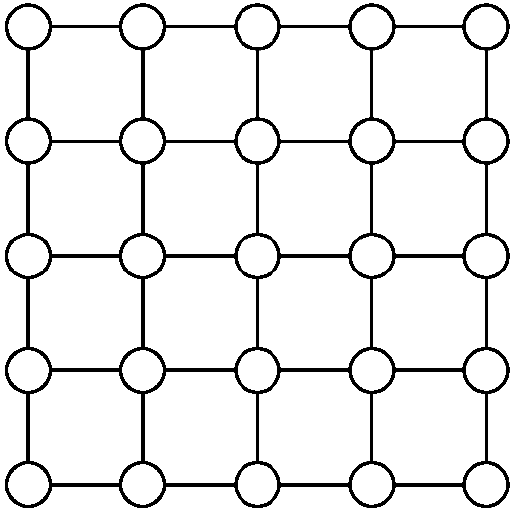
\includegraphics[width=100pt]{pics/graph_ising.png}
 \caption{Vertices $V$ and neighborhood $K$: lattice graph structure.}\label{fig:graph}
 \end{center}
 \end{figure}

\newpage
\item Consider a binary image of height $h$ and width $w$, which is represented as a $d=hw$ dimensional
vector $\bfx=(x_1,\ldots,x_d)$. For a convenience, denote pixel values as $-1$ (black) and $+1$ (white), i.e.,
$\bfx\in\{-1,+1\}^d, x_i\in\{-1,+1\}, i=1,\ldots,d$.\par
However, we observe $\bfz$, an image which is  \textsl{broken} in the following way: each pixel is  independently flipped to the opposite
($-1 \leftrightarrow +1$) with a known probability $\alpha\in(0,1)$. See sample images in Fig. \ref{fig:mickey}
Thus, the probability of observing $\bfz$ if true image is $\bfx$ can be expressed as ($C_2$ is a normalization constant):
\begin{equation}
 P(\bfZ=\bfz| \bfX=\bfx)={1\over C_2}(1-\alpha)^{\lambda_2|\{i:x_i=z_i\}|}\alpha^{\lambda_2|\{i:x_i\neq z_i\}|},
\end{equation}
where $\lambda_2=1$ (it will be different later).
However, we impose some assumptions (\textsl{knowledge}) on distributions of images, namely, ``\textsl{nearby pixels
have similar values}'', what is expressed by the Ising model ($\lambda_1>0$):

\begin{equation}
P(\bfX=\bfx)={1\over C_1}\exp\left(\lambda_1 \sum_{i,j: (i,j)\in K} x_i x_j\right),
\end{equation}
where the underlying graph is $G=(V,K)$ with $V$ being all pixels and $K$ represents neighborhood of pixels
(think lattice graph structure given in Fig. \ref{fig:graph}).
\medskip\par
\textsl{(Bayesian approach)}. Having observed $\bfz$, we can write a posteriori distribution
  \begin{eqnarray}
  \lefteqn{\pi(\bfx)= P(\bfX=\bfx| \bfZ=\bfz)=} \label{eq:XZ}\\
  & &  {1\over C}\exp\left(\lambda_1 \sum_{(i,j)\in K} x_i x_j+\lambda_2\left[|\{i:x_i=z_i\}|\ln(1-\alpha)+|\{i:x_i\neq z_i\}|\ln\alpha\right]\right).\nonumber
  \end{eqnarray}
  Now we assume that both parameters $\lambda_1, \lambda_2>0$. Note that if $\lambda_1 \gg \lambda_2$
  then $P(\bfX=\bfx| \bfZ=\bfz)$ \textsl{``pays more attention''} to $\bfx$ in which nearby pixels have similar values
  and it \textsl{``pays less attention''} to those $\bfx$ which are more similar to observed $\bfz$.
  In case $\lambda_1\ll\lambda_2$ it is the opposite.
  \medskip\par
  Show a construction of Gibbs sampler for distribution $\pi(\bfx)$ given in (\ref{eq:XZ}).




 \begin{figure}
 \begin{center}
 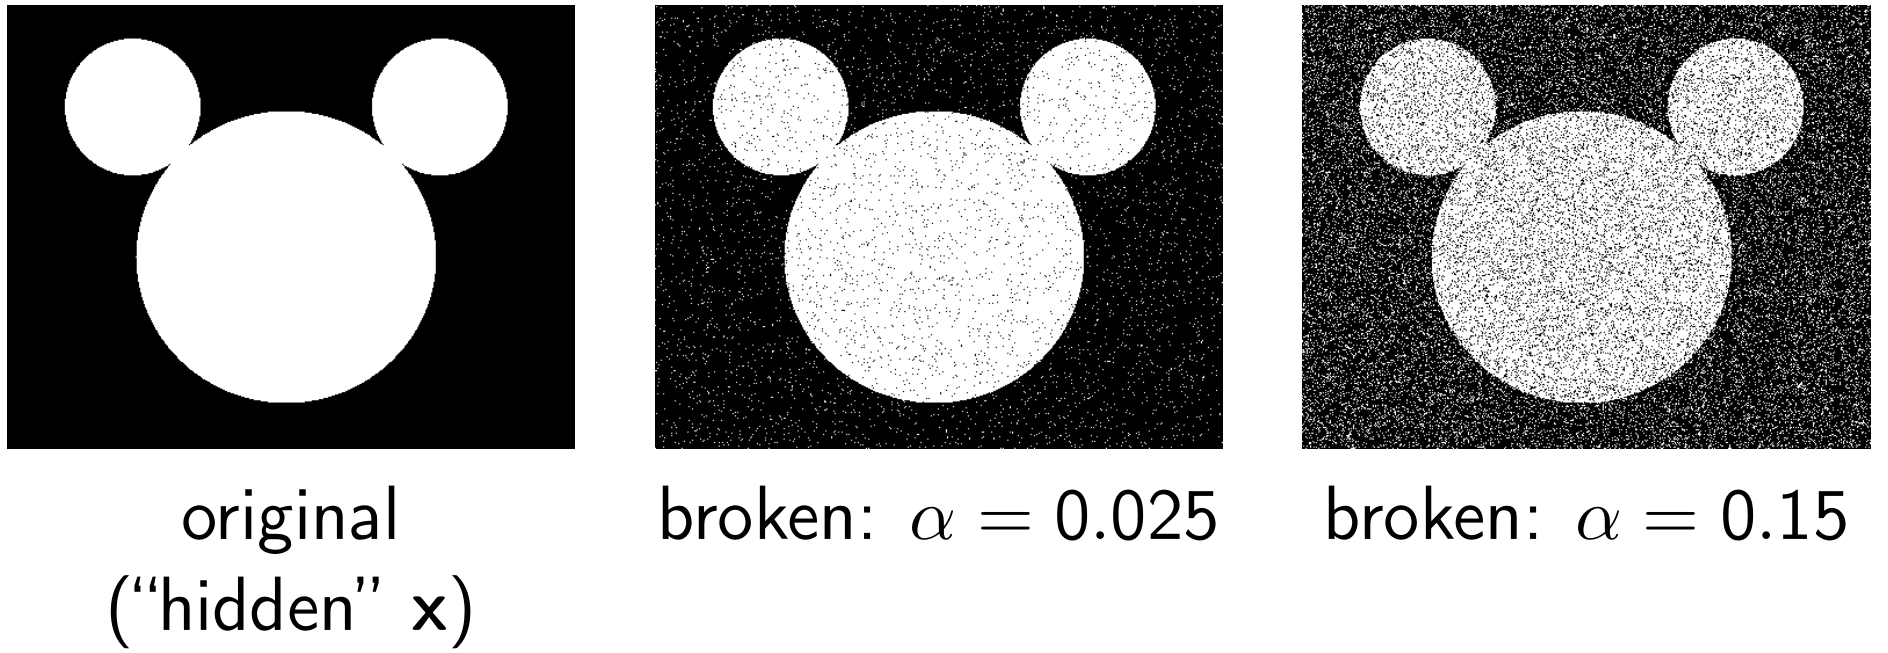
\includegraphics[width=400pt]{pics/mickey_mouse_broken.png}
 \caption{Original image (left) and broken images (middle, right).}\label{fig:mickey}
 \end{center}
 \end{figure}



\end{enumerate}



\end{document}
